%% tex/nondeterminism.tex
%% Copyright 2019 Andrea Berlingieri
%
% This work may be distributed and/or modified under the
% conditions of the LaTeX Project Public License, either version 1.3
% of this license or (at your option) any later version.
% The latest version of this license is in
%   http://www.latex-project.org/lppl.txt
% and version 1.3 or later is part of all distributions of LaTeX
% version 2005/12/01 or later.
%
% This work has the LPPL maintenance status `maintained'.
%
% The Current Maintainer of this work is Andrea Berlingieri.
%
% This work consists of all files listed in manifest.txt
\chapter{Complessità non deterministica}

\section{Macchine di Turing non deterministiche}

Vediamo un altro modello di calcolo interessante, quello delle Macchine di Turing non
deterministiche.

Una MdT non deterministica è definita in modo analogo alla versione deterministica, con la sola
differenza che la funzione di transizione $\delta$ è multivalore:
\begin{equation*}
    \delta \subseteq Q \times \Sigma^{k} \times \powerset{Q \times \Sigma^{k} \times \set{L,R}^{k}}
\end{equation*}

In altri termini nella MdTN invece di avere una sola quintupla per ogni coppia stato-carattere ne
abbiamo un insieme finito. In un certo senso è come se avessimo un programma che, invece di avere
una singola istruzione con cui continuare, ha un insieme finito di istruzioni tra cui scegliere per
proseguire la sua computazione.

È semplice da definire formalmente, basta modificare la definizione della macchina deterministica.
La macchina deterministica è in un certo senso più difficile da definire formalmente rispetto alla
versione non deterministica, dato che la si può definire ponendo dei vincoli alla definizione di
quest'ultima.

La macchina deterministica rappresenta un caso particolare della macchina non deterministica dove la
scelta della quintupla è univoca. Se qualcosa è calcolabile da una macchina deterministica lo è
anche da una non deterministica. Di conseguenza le classi deterministiche sono contenute nelle
corripondenti classi non determistiche. Ad esempio, $\PClass \subseteq \NPClass$, $\PSPACE \subseteq
\NPSPACE$, etc.

Definire la MdTN è semplice. È più complicato definire cosa calcola la MdTN. In una MdTN è
facile capire che ci sono più computazioni possibili. Quale sia però il risultato calcolato dalla
macchina non è ovvio.

Noi ci restringiamo a considerare solamente macchine decisionali, ovvero che rispondono sì/no.
Queste ci sono sufficienti perché siamo interessati a riconoscere linguaggi. Le nostre macchine
terminano con risposta booleana.

Quando possiamo affermare che una stringa è accettata da una MdTN? Abbiamo due criteri. Una stringa
può essere accettata dalla MdTN se, qualunque computazione della macchina venga fatta, la stringa
viene sempre accettata, oppure può essere accettata se esiste una computazione che accetta la
stringa. A noi interessa la seconda definizione, quella della ``macchina fortunata'': ogni volta che
abbiamo una scelta la nostra macchina fa quella giusta.

%Se esiste una computazione della MdTN che porta al riconoscimento la stringa è considerata
%riconosciuta. // Ripetizione

La computazione della macchina può essere rappresentata da un grafo.

\begin{figure}[h]
    \begin{center}
        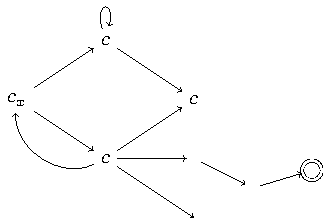
\includegraphics{./img/nondeterminism/MdTN.pdf}
        \caption{Grafo delle computazioni di una MdTN}
    \end{center}
\end{figure}

Il grafo è diretto non necessariamente aciclico. Il numero di scelte è finito e definito dalla
macchina (dal programma), che è finita. Il grafo non è neanche necessariamente finito, dato che
possono esistere computazioni che non terminano non cicliche.

Ci porremo più avanti il problema di simulare la MdTN, e qui ci tornerà utile questo grafo, detto
grafo delle computazioni.

Alcuni cammini nel grafo portano a stati finali accettanti, altri no, altri possono andare avanti
indefinitamente. A noi basta che esista un cammino che porti ad una configurazione di accettazione
per riconoscere una stringa.

%La nostra definizione di accettazione ci permetterà di avere delle relazioni con l'esistenza di un
%certificato.

Consideriamo $\SAT$. Come funzionerebbe la MdTN per $\SAT$? Noi dobbiamo prendere una formula
proposizionale e decidere se questa è soddisfacibile. La nostra macchina comincia a leggere la
formula e trova come prima variabile proposizionale, ad esempio, $A$. $A$ è vera o falsa? La
macchina ``tira una moneta'' e decide il valore di verità di $A$. Dopodiché la macchina va avanti.
Questo processo continua fino alla fine della formula. Se la formula è soddisfacibile esiste almeno
una computazione fortunata che indovinerà l'assegnazione giusta di valori di verità alle variabili
proposizionali.

Alla macchina non deterministica basta una scansione lineare della formula, e quindi riesce a
risolvere $\SAT$ in tempo lineare, a patto di prendere la strada giusta. $\SAT$ è risolvibile in
tempo polinomiale non deterministico da una MdTN. Questa sarà anche il modo in cui definiremo la
classe $\NPClass$.

\section{Complessità non deterministica}

Dobbiamo definire quali sono il tempo e lo spazio consumati dalla MdTN durante una computazione. Se
la macchina accetta l'input esiste una computazione accettante. Se la risorsa che consideriamo è il
tempo noi prendiamo il tempo della computazione accettante più corta. In termini del grafo delle
computazioni prendiamo il più corto cammino accettante della MdTN e la lunghezza di quel cammino è
il numero di passi richiesto per riconoscere una stringa $x$. Questo numero rappresenta quindi il
tempo richiesto dalla macchina. Indichiamo il tempo richiesto dalla MdTN $M$ su input $x$ con
$\textit{time}_{M}(x)$.

Analogamente per lo spazio prendiamo lo spazio minimo tra gli spazi richiesti dalle computazioni
accettanti. Tuttavia bisogna fare attenzione al come calcoliamo lo spazio richiesto da una
computazione. Questo corrisponde al massimo spazio usato in una configurazione della computazione.
Dobbiamo considerare il ``minimo dei massimi''. Indichiamo lo spazio richiesto dalla MdTN $M$ su
input $x$ con $\textit{space}_{M}(x)$.

Le funzioni $t_{M}$ e $s_{M}$ sono definite identicamente a come lo erano nel caso deterministico, a
patto di usare le nozioni di $\textit{time}$ e $\textit{space}$ appena definite. Un discorso analogo
di applica alle definizioni di $\NTIME(f)$ e $\NSPACE(f)$.

Possiamo definire le classi $\NPClass$, $\NEXP$, $\NLOGSPACE$ e $\NPSPACE$ in maniera identica a
come abbiamo definito le corrispondenti classi deterministiche, avendo cura di usare $\NTIME$ al
posto di $\DTIME$ e analogamente per lo spazio.

Possiamo formalizzare quanto detto prima sulla relazione tra macchine di Turing deterministiche e
non deterministiche con il seguente teorema.
\begin{thm}
    Per ogni $f: \Nat \to \Nat$
    \begin{equation*}
        \DTIME(f) \subseteq \NTIME(f) \land \DSPACE(f) \subseteq \NSPACE(f)
    \end{equation*}
\end{thm}
La dimostrazione è ovvia essendo la macchina di Turing determinstica un caso particolare della
macchina non deterministica.

%(Abbiamo saltato la riduzione dei nastri)

\section{Simulazione del non determinismo}

Vogliamo stabilire delle relazioni tra la MdTN e la corrispondente macchina deterministica. Per
stabilire queste relazioni una tecnica che risulta utile è pensare in termini di simulazione.
Siamo quindi interessati a teoremi che riguardano la simulazione del nondeterminismo.

Immaginiamo di avere una macchina non deterministica che riconosce un linguaggio con una certa
complessità e immaginiamo di simularla con una macchina deterministica. Se riusciamo a determinare
la complessità della simulazione rispetto alla complessità della macchina di partenza riusciamo a
dire qualcosa sulla complessità del riconoscimento del linguaggio in modo deterministico.

C'è un modo interessante di vedere la simulazione della MdTN: consideriamo il grafo delle
computazioni di una MdTN. Per simulare la macchina in modo deterministico ci basta trovare un
algoritmo deterministico di visita dei cammini del grafo. Dobbiamo fare un'esplorazione completa,
dato che possono esistere in generale cammini di riconoscimento migliori di uno già trovato.
Dobbiamo fare una qualche visita astuta per effettuare la simulazione.

%Slide 89

In generale quando vogliamo stabilire delle relazioni tra classi deterministiche e classi non
deterministiche usiamo classi di risorse diverse. Ad esempio, avendo un bound di tempo alla
complessità della MdTN diciamo qualcosa riguardo alla complessità in spazio della simulazione
deterministica. Il primo teorema che vediamo mostra questo.

\subsection{Simulazione di una macchina non deterministica con un bound al tempo}

Supponiamo di conoscere la complessità $O(f)$ in tempo della macchina non deterministica e ci
chiediamo quale sia la complessità in spazio della simulazione deterministica, cercando di
minimizzare l'occupazione di memoria.

Quello che dobbiamo fare è occupare il minor spazio possibile durante la nostra visita del grafo
delle computazioni. La visita in ampiezza non è la migliore scelta in questo caso, dato che in
generale potremmo avere una frontiera attiva dei nodi da visitare molto ampia che non ci è
necessaria.

Abbiamo che la MdTN lavora in $\NTIME(f)$. Abbiamo che $f$ rappresenta la lunghezza massima dei
cammini da esplorare, dato che sappiamo che nostra macchina non deterministica riconosce il nostro
linguaggio in tempo $O(f)$. Rispetto a questa lunghezza dei cammini il numero di nodi che possiamo
avere cresce in generale esponenzialmente: se avessimo, ad esempio, per ogni nodo una scelta
binaria, avremmo $2^{n}$ nodi.

Consideriamo una visita in profondità. Esploriamo il primo cammino, con lunghezza $O(f(|x|))$.
Quante configurazioni incontriamo? $O(f(|x|))$. Possiamo dire qualcosa sulla dimensione di queste
configurazioni?

Abbiamo che anche per la MdTN il tempo fa da bound allo spazio. Per ogni configurazione l'aspetto
che influisce di più sull'occupazione di spazio è la dimensione dei nastri. I nastri crescono, al
massimo, in modo lineare rispetto al tempo. La dimensione dei nastri è bound da $O(f(|x|))$. Per
memorizzare la catena della configurazioni ci serve $O((f(|x|))^{2})$ spazio.

Questo è lo spazio richiesto per la visita di un ramo del grafo. Tuttavia il ramo che stiamo
visitando potrebbe essere un ramo di fallimento, oppure un ramo che diverge. Nel caso fossimo in uno
di questi due casi, una volta raggiunta una configurazione di fallimento o una volta che abbiamo
raggiunto il bound in tempo della MdTN senza accettare possiamo tornare indietro lungo il ramo alla
prima configurazione dove ci è ancora possibile fare una scelta e effettuarne una diversa.
Procediamo quindi per backtracking. In ogni caso l'occupazione di tutti i cammini che esploriamo ha
gli stessi upper bound dati per il primo cammino.

Con una simulazione di questo tipo lo spazio richiesto dalla simulazione deterministica della MdTN
è dell'ordine di $O(f^{2})$.

Possiamo però fare di meglio. Perché?

In generale come facciamo a risparmiare spazio? Possiamo rendere implicite le rappresentazioni
esplicite dei dati, attraverso una descrizione compatta che prenderà tempo al momento
dell'esecuzione ma ci permetterà di risparmiare spazio. Al costo del tempo risparmiamo spazio.
Tutto ciò che ci è oneroso dal punto di vista della memoria lo rendiamo implicito attraverso una
sintesi compatta (ad esempio una compressione). Quando, in fase di esecuzione, avremo bisogno del
dato ci basterà spendere un pò di tempo per estrarlo dalla sua descrizione.

Abbiamo una tecnica analoga per risparmiare tempo a costo dello spazio. Pensiamo, ad esempio, alla
programmazione dinamica con memoization. Manteniamo una tabela per memorizzare le soluzioni dei
sottoproblemi. Quando ci serve una soluzione ad un sottoproblema possiamo guardare la tabella e, nel
caso il sottoproblema sia già stato risolto, ottenere subito il risultato richiesto. Se questo non
è il caso risolviamo il sottoproblema e memorizziamo la soluzione in tabella per usi futuri.

Tempo e spazio sono due risorse ``complementari''. Non si può, allo stesso tempo, ottimizzare il
tempo e lo spazio. Ottimizzare in tempo richiede spendere in spazio e viceversa.  Di solito siamo
portati a pensare a ottimizzazioni del tempo, senza considerare lo spazio.

Quello che occupa più spazio nella nostra visita dei cammini è la memorizzazione esplicita della
catena di configurazioni. Possiamo dare una descrizione del cammino che prendiamo nel grafo molto
più compatta, ad esempio come sequenza di scelte fatte dalla configurazione iniziale. Possiamo
etichettare ogni scelta nel cammino con un numero e salvarci le etichette del nostro cammino.
L'unica informazione che ci serve per definire il cammino è la sequenza delle scelte prese. Nel
caso dovessimo fare backtracking possiamo ripercorrere tutte le scelte del cammino corrente fino
alla scelta da rivedere e cambiare scelta. Considerando tutte le possibili scelte avremo considerato
tutti i possibili cammini del grafo.

Quanto ci costa memorizzare questa sequenza di scelte? L'unica configurazione che teniamo attiva è
quella finale, che è bound da $O(f(|x|))$ per il teorema tempo spazio. Le scelte sono in un range
finito fissato dalla macchina.

In definitiva ci servirà $c\cdot O(f(|x|))$ spazio per memorizzare le scelte e $O(f(|x|))$ per la
configurazione finale del cammino. L'ordine dell'occupazione di spazio della simulazione fatta in
questo modo è quindi $O(f(|x|))$. Riusciamo a fare la simulazione della MdTN in spazio $O(f(x))$.

\begin{thm}\label{thm:ntimedspace}
    Per ogni $f:\Nat \to \Nat$ costruibile in spazio maggiore o uguale all'identità:
    \begin{equation*}
        \NTIME(f) \subseteq \DSPACE(f)
    \end{equation*}
\end{thm}

Possiamo vedere la simulazione in un modo più operazionale. Dato $x$ inizializziamo due nastri di
dimensione $f(|x|)$. In un nastro memorizziamo il tape e in un altro le scelte. All'inizio
simuleremo la computazione dove la scelta che facciamo è sempre la prima. Sul nastro del tape
simuliamo la computazione della MdTN. A questo punto arriviamo in fondo in vari modi: o terminiamo
il tempo, o cerchiamo di sforare lo spazio, o ci arrestiamo con riconoscimento, o ci arrestiamo con
fallimento. In quest'ultimo caso andiamo a cambiare l'ultima scelta per fare backtracking e
rifacciamo la computazione. L'occupazione di spazio rimane dell'ordine $O(f)$. Dovremmo memorizzare
anche un timer per non sforare in tempo, ma questo ha occupazione logaritmica nel valore di $f$. Di
conseguenza l'occupazione di spazio non peggiora.

\begin{figure}[h]
    \begin{center}
        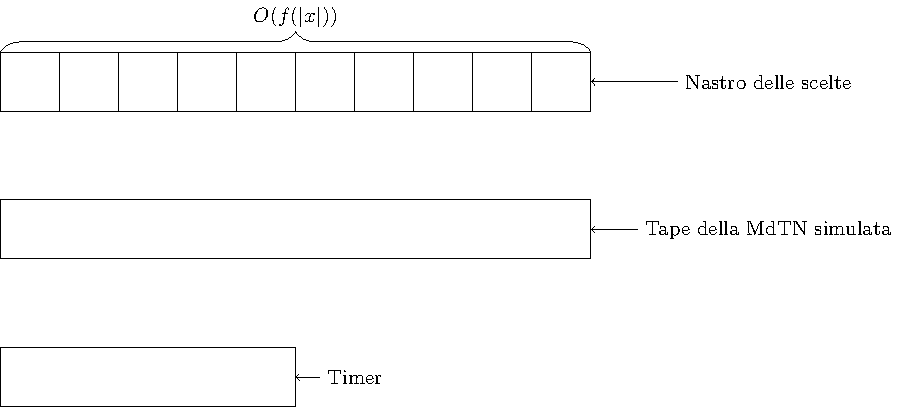
\includegraphics[scale=0.7]{./img/nondeterminism/Simulation.pdf}
        \caption{Simulazione deterministica di una MdTN con memoriazzazione delle scelte}
    \end{center}
\end{figure}

% TODO change all explicit references to "teorema tempo spazio" with a \ref to the right theorem
La simulazione del nondeterminismo non richiede un grande utilizzo di spazio. Il teorema
\ref{thm:ntimedspace} generalizza il teorema tempo spazio: non solo $\DTIME(f)$ è contenuto in
$\DSPACE(f)$, ma anche $\NTIME(f)$. Dal teorema e dall'inclusione $\DTIME(f) \subseteq \NTIME(f)$
deriva il teorema tempo spazio.

\subsection{Simulazione di una macchina non deterministica con un bound allo spazio}

Vediamo ora cosa possiamo dire della complessità in tempo della simulazione di una MdTN che lavora
con una data complessità in spazio.

Sia $M$ una MdTN che riconosce un linguaggio $\Lang \in \NSPACE(f)$ e consideriamo il suo grafo di
raggiungibilità. Possiamo fare un'ipotesi aggiuntiva su questo grafo e dire che esiste un'unica
configurazione finale di riconoscimento. Ciò è diverso dall'affermare che abbiamo un solo stato
finale di riconoscimento. Possiamo fare questa ipotesi perché in generale possiamo ``canonizzare''
tutte le configurazioni finali di una MdTN ``ripulendo'' i nastri, e ottenere una macchina con la
stessa complessità in spazio con un'unica configurazione finale. Questa operazione di
canonicalizzazione degli stati finali richiederà sicuramente del tempo ma non dello spazio
aggiuntivo.

\begin{figure}[h]
    \begin{center}
        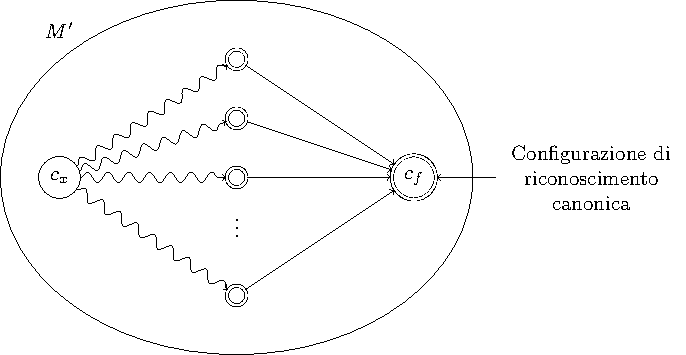
\includegraphics[scale=0.7]{./img/nondeterminism/Canonicalization.pdf}
        \caption{Canonicalizzazione di una MdTN $M$.}
    \end{center}
\end{figure}

Sotto questa ipotesi possiamo vedere la simulazione deterministica di $M$ come la ricerca di un
cammino dalla configurazione iniziale all'unica configurazione finale accettante. La complessità di
questa operazione sarà proporzionale alla dimensione del grafo delle computazioni di $M$.

Possiamo dare un upper bound alla dimensione del grafo? Sì. Cerchiamo di capire quanti sono i nodi
di questo grafo. Gli archi saranno di ordine quadratico rispetto a questa quantità. I nodi sono le
possibili configurazioni finite diverse possibili. Abbiamo che la dimensione dei nastri è $O(f)$.
Sappiamo quante sono le configurazioni possibili dato un bound allo spazio: saranno una quantità di
ordine esponenziale in $f$. Abbiamo quindi che la dimensione del grafo sarà $O(2^{cf})$.

\begin{thm}\label{thm:nspacedtime}
    Per ogni $f:\Nat \to \Nat$ costruibile in spazio maggiore esiste $c \in \Nat$ tale che
    \begin{equation*}
        \NSPACE(f) \subseteq \DTIME(2^{c(\log + f)})
    \end{equation*}
\end{thm}

Il $\log$ nell'esponenziale ci indica, come sempre, che richiediamo che $f$ sia almeno $\geq
\log(n)$. Questo perché consideriamo complessità in tempo almeno lineari.

Anche in questo caso abbiamo una generalizzazione del teorema tempo spazio. Questa generalizzazione
è stretta se supponiamo che $\DSPACE(f) \subset \NSPACE(f)$. Questo, al solito, si congettura ma
non è ancora stato dimostrato. Abbiamo che $\DSPACE(f) \subseteq \NSPACE(f)$, da cui $\DSPACE(f)
\subseteq \DTIME(2^{c(log + f)})$.

Possiamo dire che i teoremi tempo spazio valgono se immaginiamo che dalla parte sinistra delle
inclusioni abbiamo una macchina non deterministica.

Possiamo ora concludere qualcosa riguardo all'utilizzo di risorse dello stesso tipo nella
simulazione di una MdTN.

Supponiamo di avere una MdTN che lavora con complessità in $\NTIME(f)$. Per il teorema
\ref{thm:ntimedspace} abbiamo che $\NTIME(f) \subseteq \DSPACE(f)$. Per il teorema tempo spazio
$\DSPACE(f) \subseteq \DTIME(2^{cf})$, per un $c$ opportuno. Di conseguenza $\NTIME(f) \subseteq
\DTIME(2^{cf})$. Potrebbe andare meglio per casi specifici, ma l'upper bound dato è sempre valido.
Questo risultato non è tanto sorprendente, se consideriamo un tipico grafo delle computazioni di
una MdTN.

Cosa possiamo dire per lo spazio? Abbiamo sicuramente che $\NSPACE(f) \subseteq \DTIME(2^{cf})$, per
un opportuno $c$. Per il teorema tempo spazio abbiamo che $\DTIME(2^{cf}) \subseteq
\DSPACE(2^{cf})$, da cui $\NSPACE(f) \subseteq \DSPACE(2^{cf})$. Questo risultato è meno intuitivo,
dato che lo spazio è una risorsa riutilizzabile. Il tempo, invece, non lo è. Potremmo utilizzare lo
spazio già usato per una computazione per provarne un'altra. Non è ovvio che si possa fare meglio,
ma si può ed è dimostrabile. Inoltre il miglioramento è molto significativo.

\subsection{Teorema di Savitch}

\begin{thm}
    \textbf{(Teorema di Savitch).} Sia $f:\Nat \to \Nat$ una funzione costruibile in spazio e tale
    che $\log \in O(f)$. Allora
    \begin{equation*}
        \NSPACE(f) \subseteq \DSPACE(f^{2})
    \end{equation*}
\end{thm}

Simulare in modo deterministico una computazione non deterministica che richiede spazio $O(f)$ è
fattibile in spazio $O(f^{2})$.

È un teorema importante perché ha un corollario molto rilevante. Una simulazione deterministica di
una MdTN ha un overhead esponenziale in tempo, ma non in spazio. Abbiamo un overhead quadratico.

L'idea è sempre quella di fare una visita del grafo. Supponiamo di essere sotto l'ipotesi di
unicità della configurazione finale accettante. Siamo alla ricerca di un cammino che vada dalla
configurazione iniziale a quella finale cercando di occupare il minor spazio possibile. Solitamente
si adoperano due algoritmi per questa problematica: DFS e BFS. Abbiamo gia analizzato la loro
complessità in tempo, ci chiediamo quale sia la loro complessità in spazio.

Consideriamo DFS. La massima profondità di una visita è uguale al numero dei nodi, visto che
consideriamo cammini aciclici. Possiamo supporre di avere una descrizione compatta di un cammino, ma
sarà sempre lineare nel numero dei nodi in dimensione. Questo discorso si applica anche a BFS. La
frontiera che possiamo ottenere, nel caso pessimo, può avere dimensione pari al numero di nodi del
grafo. Questi due algoritmi hanno un'occupazione di memoria almeno lineare.

Esiste però un algoritmo per questa problematica concettualmente semplice ma con un'occupazione di
memoria sorprendentemente bassa: $O(\log^{2}(n))$, dove $n$ è il numero dei nodi. Questo è lo
spazio aggiuntivo richiesto, ignorando lo spazio richiesto dall'input.

L'algoritmo utilizza una funzione ricorsiva che possiamo chiamare $\REACH$. $\REACH$ prende in input
due nodi $u$ e $v$ e un parametro $i$. Supponiamo che i nodi siano stati numerati e che $u$ e $v$
siano quindi numeri. Il problema che $\REACH$ risolve è determinare se esiste un cammino da $u$ a
$v$ di lunghezza $\leq 2^{i}$.

L'idea è quella di fare una sorta di divide-et-impera. Abbiamo $u$, $v$ e cerchiamo un cammino di
lungheza $\leq 2^{i}$. Se questo esiste possiamo spezzarlo in due cammini di lunghezza $\leq
2^{i-1}$. In questo caso esiste anche un nodo $x$ ed un cammino di lunghezza $\leq 2^{i-1}$ da $u$ a
$x$ e un cammino analogo da $x$ a $v$. Tuttavia non sappiamo quale nodo sia l'$x$ che cerchiamo; di
conseguenza per trovarlo facciamo una ricerca esaustiva su tutti i possibili $x$.

\begin{figure}[h]
    \begin{center}
        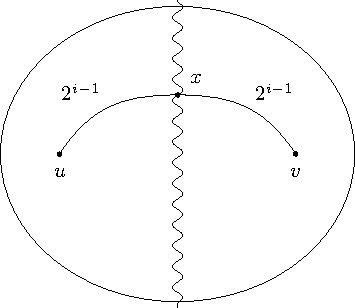
\includegraphics{./img/nondeterminism/SavitchAlgorithm.pdf}
        \caption{Possiamo dividere la ricerca di un cammino di lunghezza $\leq 2^{i}$ nella ricerca
        di due cammini di lunghezza $\leq 2^{i-1}$, utilizzando lo stesso algoritmo.}
    \end{center}
\end{figure}

Lo pseudocodice è illustrato in Algorithm \ref{algo:reach}

\RestyleAlgo{ruled}
\begin{algorithm}
%    \SetNlSty{texttt}{(}{)}
    \caption{\REACH(\textsc{Graph} $G$,\textsc{Node} $u$,\textsc{Node} $v$, \textbf{integer} $i$)}
    \label{algo:reach}
    \If {$i = 0$}
    {
        \Return{$u = v \lor (u,v) \in G.V$}
    }
    \Else
    {
        $\textbf{boolean } res \gets \textbf{false}$

        \ForEach{$x \in G.V$}
        {
            $res \gets res \lor (\REACH(G,u,x,i-1) \land \REACH(G,x,v,i-1)$
        }

        \Return{$res$}
    }
\end{algorithm}

Questo algoritmo è noto come algoritmo di Savitch.

La chiamata iniziale la faremo con un upper bound alla lunghezza massima. Poichè la lunghezza
massima di un cammino aciclico in un grafo è $n$, come valore iniziale per $i$ useremo $\log(n)$:
infatti $2^{\log(n)} = n$.

Discutiamo la complessità in spazio di questo algoritmo. Supponiamo di implementare le chiamate
ricorsive dell'algoritmo mediante uno stack di record di attivazione. Ciò che influisce
sull'occuazione di spazio è il numero massimo di chiamate annidate che possiamo avere e la
dimensione massima dei record di attivazione. Qual è il numero massimo di chiamate annidate? $i$,
dato che ad ogni chiamata l'input decresce. Abbiamo che $i \leq \log(n)$.

Possiamo dare un upper bound anche alla dimensione dei record di attivazione. Nei record di
attivazione abbiamo, in genere, l'input, l'output e le variabili locali. Le variabili di questa
procedura sono, ad esempio, \textit{res} e $x$. Qual'è la dimensione di queste variabili? I nodi
sono dei numeri e la risposta è un booleano. Per memorizzare i nodi ci basta $O(\log(n))$, mentre
per memorizzare la risposta ci è sufficiente uno spazio costante. Avremo un numero costante $k$ di
variabili locali, ma questo non influisce sulla complessità.

Di conseguenza la dimensione richiesta per capire se due nodi sono raggiungibili è dato da $i\cdot
k\log(n) \leq k\log^{2}(n)$, ovvero $O(\log^{2}(n))$. Allo stato dell'arte non si riesce a fare di
meglio a livello di occupazione di spazio.

Qual'è la complessità in tempo di questa procedura? Ricordiamo che abbiamo un trade-off quando
ottimizziamo lo spazio: questa operazione ci costa in tempo. Scriviamo la relazione di ricorrenza:
il tempo $t$ richiesto al passo $i$ è dato da:
\begin{equation*}
    t_{i} =
    \begin{cases}
        \case{d}{se $i = 0$}\\
        \case{N\cdot 2t_{i-1}}{altrimenti}\\
    \end{cases}
\end{equation*}

Il numero di chiamate è $i \leq \log(N)$. Abbiamo quindi una complessità $O((N\cdot 2)^{\log(N)})
= O(N^{\log(N)}2^{\log(N)}) = O(N\cdot N^{log(N)}) = O(N^{\log(N)+1})$. Potevamo ottenere un bound
simile con il teorema tempo spazio.

È un problema aperto della teoria della complessità riuscire a trovare, se esiste, un algoritmo
che stia ``a metà'' tra questo algoritmo, che ottimizzza lo spazio, e un tipico algoritmo di visita
che ottimizza il tempo.

Tornando alla dimostrazione del teorema di Savitch, sappiamo che riusciamo a fare la ricerca di un
cammino dalla configurazione iniziale a quella finale con uno spazio limitato. Qual è la dimensione
del grafo? Se $f$ è il bound asintotico allo spazio abbiamo un numero di configurazioni
$O(2^{cf})$, per un $c$ opportuno. Con questa dimensione del grafo e utilizzando l'algoritmo di
Savitch abbiamo una complessità $\log^{2}(2^{cf}) = (cf)^{2}$, ovvero $O(f^{2})$.

% TODO rivedi registrazione su questo punto
Questa complessità è tale se nell'occupazione di spazio consideriamo solo quello aggiuntivo
richiesto per la computazione, ignorando quello richiesto per memorizzare l'input. Possiamo fare
questa ipotesi perché possiamo lavorare con il grafo in maniera implicita. L'unico momento in cui
ci serve esplicitamente il grafo è nel caso base dell'algoritmo. Abbiamo una configurazione
$c_{u}$, una configurazione $c_{v}$ e ci chiediamo se si può andare, in un passo, da $c_{u}$ a
$c_{v}$. Dal punto di vista dell'occupazione in spazio questo richiede uno spazio uguale al massimo
tra quelli richiesti da $c_{u}$ e da $c_{v}$. L'importante è fissare $M$, di dimensione costante
che dipende dal programma.

Cosa ci dice questo teorema su $\NPSPACE$? Supponiamo di avere un polinomio, ad esempio $n^{2}$.
Supponiamo di voler riconoscere un linguaggio $\Lang \in \NSPACE(n^{2})$. Per il teorema di Savitch
abbiamo che lo stesso linguaggio sta in $\DSPACE(n^{4})$. In generale il quadrato di un polinomio è
ancora un polinomio. Di conseguenza abbiamo che $\NPSPACE \subseteq \PSPACE$. Poichè le macchine
deterministiche sono un caso particolare di macchine non deterministiche, come ulteriore conseguenza
abbiamo che $\NPSPACE = \PSPACE$.

Questo è l'equivalente, a livello dello spazio, del problema $\PClass$ vs $\NPClass$. Se avessimo
un risultato simile per il tempo, ad esempio $\NTIME(f) \subseteq \DTIME(f^{20})$, potremmo
concludere $\PClass = \NPClass$. Tuttavia un risultato del genere probabilmente non è dimostrabile.

Il motivo per cui l'occupazione di spazio dell'algoritmo di Savitch è compatta è che non
memorizziamo nulla delle computazioni già fatte, mentre la complessità in tempo rimane elevata
dato che per ogni coppia di nodi $u$ e $v$ del grafo sarà ripetuta varie volta l'interrogazione
``il nodo $u$ è raggiungibile dal nodo $v$?''.

Non è possibile risparmiare il tempo di queste computazioni memorizzando, ad esempio, i risultati
delle varie interrogazioni in una tabella. Questo perché il numero dei nodi è esponenziale nella
complessità in spazio. La dimensione di questa tabella sarebbe anch'essa esponenziale e non
riusciremmo a lavorare in uno spazio quadratico in $f$. Come sempre se vogliamo risparmiare in
spazio dobbiamo essere disposti a ``spendere'' in tempo, e viceversa.

%Slide 103
\subsection{Gerarchie di complessità}

Possiamo, dati i risultati sulle computazioni non deterministiche, rappresentare le relazioni di
inclusioni mediante la figura \ref{nondeterminism:img:complexity_hierarchy}:

\begin{figure}[h]
    \begin{center}
        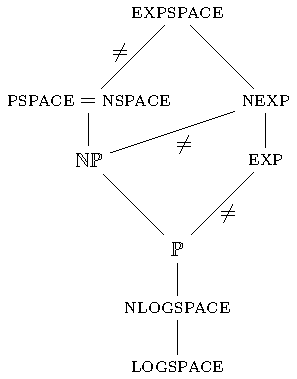
\includegraphics{./img/nondeterminism/Hierarchies.pdf}
        \caption{Rappresentazione delle relazioni di inclusioni note tra alcune classi di
        complessità.}
        \label{nondeterminism:img:complexity_hierarchy}
    \end{center}
\end{figure}

Il significato degli archi e dei segni di disuguaglianza è lo stesso che abbiamo dato per la figura
\ref{timespacehierarchies:img:detclassesrelations}.

Abbiamo che $\LOGSPACE \subseteq \NLOGSPACE$ perché le macchine deterministiche sono un caso
particolare di quelle non deterministiche. Abbiamo inoltre che $\NLOGSPACE \subseteq \PClass$ per il
teorema \ref{thm:nspacedtime}. Sappiamo che $\PClass \subset \EXP$ per il teorema della gerarchia in
tempo, e analogamente abbiamo che $\NPClass \subset \NEXP$. Sappiamo che $\NPClass \subseteq \PSPACE$
per il teorema \ref{thm:nspacedtime} e sappiamo che $\PSPACE = \NPSPACE$ per il teorema di Savitch.
Sappiamo infine che $\PSPACE \subset \EXPSPACE$ per il teorema della gerarchia e che $\NEXP
\subseteq \EXPSPACE$ per il teorema \ref{thm:nspacedtime}.

L'inclusione stretta tra $\NPClass$ e $\NEXP$ non è ovvia. In effetti si può dimostrare che i
teoremi della gerarchia sono generalizzabili al caso non deterministico, e questo giustifica questa
relazione tra le due classi.
